\documentclass[12pt]{article}
\usepackage{amsmath, amssymb}
\usepackage{tikz}
\usetikzlibrary{patterns}

\begin{document}

\begin{figure}[h]
    \centering
    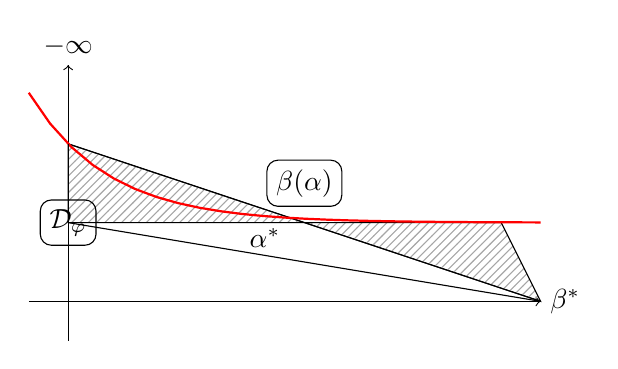
\begin{tikzpicture}
        % Axes
        \draw[->] (-0.5, 0) -- (6.0, 0) node[right] {$\beta^*$};
        \draw[->] (0, -0.5) -- (0, 3.0) node[above] {$-\infty$};
        
        % Lines
        \draw[dashed] (0, 3) -- (0, 2);
        \draw (0, 2) -- (6, 0);
        
        \draw[pattern=north east lines, pattern color=gray!70] (0, 2) -- (6, 0) -- (5.5, 1) -- (0, 1) -- cycle;
        
        \draw[red, thick, domain=-0.5:6] plot (\x, {1 + exp(-\x)});
        \draw[black, thin] (0, 1) -- (0, 2);
        \draw[black, thin] (0, 1) -- (6, 0);
        
        % Labels
        \node at (3, 1.5) [draw, rounded corners] {$\beta(\alpha)$};
        \node at (0, 1) [draw, rounded corners] {$\mathcal{D}_\varphi$};
        \node at (2.5, 0.8) [] {$\alpha^*$};
        \node at (5.5, 0.2) [] {};
        
    \end{tikzpicture}
    \caption{Construction of $\beta(\alpha)$ in Lemma \ref{Lem_Aux4} (compared to Lemma \ref{Lem_AuxL2})}
    \label{fig:construction_beta_alpha}
\end{figure}

In Lemma \ref{Lem_Aux4}, the construction of $\beta(\alpha)$ changes slightly compared to Lemma \ref{Lem_AuxL2}.
\end{document}